%===============================================================================
% ifacconf.tex 2022-02-11 jpuente  
% 2022-11-11 jpuente change length of abstract
% Template for IFAC meeting papers
% Copyright (c) 2022 International Federation of Automatic Control
%===============================================================================
\documentclass{ifacconf}

% \usepackage{hyperref}
\usepackage{graphicx}      % include this line if your document contains figures
\usepackage{natbib}        % required for bibliography
\usepackage{comment}
\usepackage{amsmath}
\usepackage{amssymb}
\usepackage[dvipsnames]{xcolor}

\usepackage{subfig}
\usepackage{kotex}
\usepackage{tikz}

\usepackage{lipsum} % for dummy text
\usepackage{multirow}
\usepackage{multicol}

\usepackage{algorithm}
\usepackage{algpseudocode}

\usepackage{xurl}

% ============================================
%         GENERAL MACROS
% ============================================
\newcommand{\template}{template}
\newcommand{\KHCH}[1]{{\color{RoyalPurple} [KH: #1]}} % Kyunghwan's
\newcommand{\JYKI}[1]{{\color{red} [JY: #1]}} % Jiyun's
\newcommand{\MSRY}[1]{{\color{Peach} [MS: #1]}} % Myeongseok's 
\newcommand\eg{\textrm{e.g.,\ }}
\newcommand\ie{\textrm{i.e.,\ }}
\definecolor{my_cyan}{rgb}{0.0, 1.0, 1.0}

\newcommand{\colorLine}[2]{[\tikz[baseline=(current bounding box.base)]{\draw[color=#1,
#2,line width=2pt] (0,3pt) -- (1.5em,3pt);}]}
% colors
% https://latexcolor.com % color list
\definecolor{airforceblue}{rgb}{0.36, 0.54, 0.66}
\definecolor{awesome}{rgb}{1.0, 0.13, 0.32}
\definecolor{darkcyan}{rgb}{0.0, 0.545, 0.545}
\newcommand{\ctxt}[2]{{\color{#1}{#2}\color{black}}}
\newcommand{\cred}[1]{{\ctxt{awesome}{#1}}}
\newcommand{\cblue}[1]{{\ctxt{airforceblue}{#1}}}

\begin{comment}
L2 Norm of Tracking Error:
C1: 1.3456
C2: 1.2804
C3: 6.8005
Improvement over C3:
C1: 80.21 %
C2: 81.17 %
\end{comment}

\newcommand{\oneErr}{{1.3456}}
\newcommand{\twoErr}{{1.2804}}
\newcommand{\threeErr}{{6.8005}}

\newcommand{\impOne}{{80.21}}
\newcommand{\impTwo}{{81.17}}

% ============================================
%         MATH MACROS
% ============================================
% \input{\template/macros/macros_math.tex}
\newcommand\R{\mathbb{R}}
\newcommand\N{\mathbb{N}}

\newcommand*{\mv}[1]{\boldsymbol{#1}} % my vector
\newcommand*{\mm}[1]{\boldsymbol{#1}} % my matrix
\newcommand*{\norm}[1]{\lVert #1 \rVert} % euclidean norm

\DeclareMathOperator{\myvec}{{vec}}       % vectorization
\DeclareMathOperator{\myproj}{{Proj}}   % projection
\DeclareMathOperator{\mysat}{{sat}}       % saturation
\DeclareMathOperator{\myrow}{{row}}       % row of a matrix
\DeclareMathOperator{\mycol}{{Col}}       % column of a matrix
\DeclareMathOperator{\mysym}{{sym}}       % symmetric part of a matrix
\DeclareMathOperator{\mydiag}{{diag}}     % diagonal matrix
\DeclareMathOperator{\mysign}{{sign}}     % sign function
\DeclareMathOperator{\mypoly}{{Poly}}     % polynomial

% ============================================
%         FRACTIONS
% ============================================
\newcommand\der{\mathrm d}
\newcommand*{\ddt}{
   \frac{\der}{\der t}
}
\newcommand*{\ddtt}{
   \tfrac{\der}{\der t}
}
\newcommand*{\ddttddtt}{
   \tfrac{\der^2}{\der t^2}
}
\newcommand*{\ddfrac}[2]{
   \frac{\der {#1}}{\der {#2}}
}
\newcommand*{\ddtfrac}[2]{
   \tfrac{\der {#1}}{\der {#2}}
}
\newcommand*{\ppfrac}[2]{
   \frac{\partial {#1}}{\partial {#2}}
}
\newcommand*{\pptfrac}[2]{
   \tfrac{\partial {#1}}{\partial {#2}}
}

%===============================================================================
\begin{document}
\begin{frontmatter}

\title{
   % Vector-Space Optimization for Contraction Theory-Based Control Design
   Vector-Space Optimization Framework Based on Projected Contraction Condition for Control Design with Input Saturation 
   \thanksref{footnoteinfo}
} 
% Title, preferably not more than 10 words.

\thanks[footnoteinfo]{
   This work was supported in part by the National Research Foundation of Korea (NRF) grant funded by the Korea government (MSIT) (RS-2025-00554087)
}

\author[First]{Myeongseok Ryu} 
\author[First]{Kyunghwan Choi} 
\author[Second]{Sesun You}

\address[First]{
   Korea Advanced Institute of Science and Technology (KAIST), 
   Daejeon 34051, South Korea (e-mail: \{dding\_98, kh.choi\}@kaist.ac.kr)}
\address[Second]{
   Incheon National University, 
   Incheon 22012, South Korea (e-mail: yousesun@inu.ac.kr)}

\begin{abstract}                % Abstract of 50--100 words
   Conventional feedback control design based on contraction theory typically requires matrix-valued contraction metrics, which can limit real-time applicability as the system dimension increases and make direct handling of input saturation nontrivial.
   To address these issues, we project the contraction condition onto the instantaneous trajectory-error direction and introduce the metric-weighted error vector as the optimization variable.
   This yields a lower-dimensional formulation that avoids direct optimization over the full matrix-valued metric and enables input saturation constraints to be incorporated directly.
   Additionally, an energy-based constraint is introduced to resolve the scale ambiguity of condition-number minimization and maintain sufficient control effort.
   The effectiveness of the proposed method is validated through numerical simulations using the Lorenz system.
\end{abstract}

\begin{keyword}
   Contraction theory, 
   optimization-based control,
   input saturation
   % energy-based control
\end{keyword}

\end{frontmatter}
%===============================================================================

\section{Introduction}

\subsection{Motivation}

Besides the traditional Lyapunov stability theory, contraction theory provides a powerful framework for analyzing nonlinear systems from an incremental stability perspective.
Rather than studying convergence to a fixed equilibrium point, contraction theory examines whether infinitesimally close trajectories exponentially converge to each other under a Riemann metric, called a contraction metric \citep{LOHMILLER:1998aa}.
Contraction theory has been extended to control and observer design, as reviewed in \citep{Tsukamoto:2021aa} and \citep{Bernard:2022aa}, respectively.

Specifically, control contraction metrics (CCMs) have been developed for feedback control design, providing universal stability certificates by introducing convex feasibility problems \citep{Manchester:2014aa,Manchester:2017aa}.
In CCM-based control design, the contraction metric is typically constructed over a prescribed operating domain in advance, often through gridding, sampling, or finite-dimensional parameterization.
Using the obtained contraction metric, a feedback control law can be obtained by integrating a differential feedback law along a shortest path, called a geodesic, between the current and the desired trajectories in the Riemannian space defined by the contraction metric.

However, enforcing the contraction condition over an entire operating domain can be computationally demanding, and the burden can increase rapidly with the dimension and size of the operating region.
Moreover, the resulting metric is tied to the selected domain and discretization, so the design may need to be repeated when the operating region or system configuration changes.
These limitations motivate step-wise formulations that compute a contraction metric at each time instant, rather than constructing a global metric over the full domain offline.

Among recent developments in contraction theory-based control, Tsukamoto {\etal} proposed ConVex optimization-based Steady-state Tracking Error Minimization (CV-STEM) \citep{Tsukamoto:2019aa}.
CV-STEM is a systematic framework for contraction metric calculation that solves a linear matrix inequality (LMI) optimization problem to minimize the steady-state tracking error bound in the presence of bounded disturbances at each time instant.
% Unlike conventional CCM-based approaches that construct a global metric over a prescribed domain offline, CV-STEM computes the contraction metric at each time instant for the current state and desired trajectory.
The framework has been developed in both state-dependent coefficient (SDC)-based and CCM-based formulations \citep{Tsukamoto:2021aa}.
In the SDC-based formulation, the error dynamics are transformed into a linear parameter-varying (LPV) system using the SDC formulation, and the contraction metric is directly applied as a feedback gain for the trajectory error.
In the CCM-based formulation, the offline-computed CCM is substituted with the obtained contraction metric at each time instant, and the control law is obtained similarly to \citep{Manchester:2017aa}.
CV-STEM has demonstrated its effectiveness and has been extended to various systems, including stochastic systems \citep{Tsukamoto:2021ad} and uncertain systems \citep{Tsukamoto:2021af}.

Despite these advances, CV-STEM still relies on matrix-space LMI optimization problems when the metric is computed at each time instant.
For an $n$-dimensional system, the contraction metric is an $n\times n$ symmetric positive definite matrix.
Thus, the number of optimization variables grows quadratically with the system dimension and the scalability of online contraction-metric computation can be limited for high-dimensional systems.
Hence, it is desirable to reduce the dimension of the optimization variable to enhance the scalability.
% Although some studies have proposed offline approximation of the contraction metric using deep neural networks (DNNs) \citep{Tsukamoto:2021ae,Tsukamoto:2021ac}, it is desirable to reduce the dimension of the optimization variable without relying on offline approximation.

Moreover, there has been limited consideration of input saturation in conventional contraction theory-based control design.
For example, in \citep{Tsukamoto:2019aa}, the input saturation constraint is considered in a conservative manner by limiting the maximum norm of the control input.
This may lead to the infeasibility of the optimization problem when the input saturation constraint is imposed too conservatively.
In addition, if the input saturation effect is not properly handled, the control performance may degrade, and invalidate the nominal stability certificate \citep{Ryu:2025aa}.

% Another issue arises from the condition-number objective used in LMI optimization problems.
% Since the steady-state tracking-error bound is proportional to the condition number of the contraction metric, the objective is to minimize the condition number.
% However, the condition number is invariant under positive scaling of the contraction metric, and therefore condition-number minimization alone does not uniquely determine the magnitude of the metric.
% Consequently, the resulting feedback gain and control effort can become ambiguous: different scaling of the metric can yield the same condition number but different control magnitudes.

% There is also the issue of an ill-posed problem in the objective function minimizing the condition number of the contraction metric, which is proportional to the steady-state error bound.
% Since the condition number is scale-invariant, there exist an infinite number of solutions for the contraction metric that yield the same condition number.
% In conventional approaches, this issue has been tackled by introducing a scaling parameter for the contraction metric and tuning it with weighting factors in the objective function \citep{Tsukamoto:2019aa,Tsukamoto:2021ae}.
% However, this approach may determine insufficient control effort to achieve the desired trajectory or lead to excessive control effort.

Motivated by these observations, this paper develops a vector-space optimization framework based on a projected contraction condition.
The key idea is to optimize a metric-weighted error vector, which is the feedback-relevant action of the contraction metric, instead of directly solving for the full matrix-valued metric.
This also allows input constraints and scale regulation to be handled in the same vector-space optimization framework.

% \cred{이거도 마찬가지임}
% On the other hand, by formulating the problem in vector space rather than matrix space, flexibility in handling various constraints, including nonlinear input and state constraints, can be improved.
% In addition, the dependency of computational complexity on the system dimension can be alleviated.
% If the contraction metric is utilized as a feedback gain for the trajectory error, the contraction metric can be projected onto the trajectory error vector space.
% This allows us to simplify the contraction metric calculation from matrix-space optimization to vector-space optimization within a lower-dimensional effective space.

% To the best of our knowledge, there has been no previous work that projects the contraction constraints onto a vector space to reduce the dependency on the system dimension for contraction metric calculation.
% Moreover, input saturation has not been actively considered in conventional contraction theory-based control design.
% Hence, the main objective of this paper is to simplify the contraction metric calculation from matrix-space optimization to vector-space optimization, while also incorporating the input saturation constraint and maintaining sufficient control effort.

\subsection{Contributions}

The main contributions of this paper are:
\begin{itemize}
   \item A vector-space optimization framework is proposed by projecting the contraction condition onto the trajectory error direction;
   \item By introducing the metric-weighted error vector as the optimization variable, the number of optimization variables is reduced, thereby improving scalability;
   % \item An energy-based constraint is introduced to resolve the scale ambiguity of condition-number minimization and to maintain sufficient control effort; and
   \item The input saturation constraint is directly incorporated into the proposed optimization framework, enhancing the practical applicability of the method.

   % \item The contraction metrics can be calculated in a lower-dimensional effective space by projecting the contraction constraints onto the trajectory error vector space. This significantly reduces the computational complexity of the LMI framework for contraction metric calculation, enabling real-time implementation;
   % \item The scale-invariance issues of the objective function minimizing the condition number of the contraction metric are resolved by introducing energy-based constraints to obtain locally optimal solutions and maintain sufficient control effort;
   % \item A convex input saturation constraint is incorporated into the proposed optimization framework, which handles the practical limitations of actuators; and
   % \item The robust feasibility of the proposed method is enhanced by introducing slack variables to relax the energy-based constraints, thereby avoiding infeasibility due to the input saturation constraint.
\end{itemize}

\subsection{Paper Organization}

The remainder of this paper is organized as follows.
Section \ref{sec:preliminaries} reviews the preliminaries of contraction theory.
Section \ref{sec:problem} formulates the problem of contraction theory-based control design.
Section \ref{sec:conv:lmi} discusses the conventional matrix-space optimization framework for contraction metric calculation and its limitations.
Section \ref{sec:main:results} presents the proposed vector-space optimization framework and provides an illustrative example.
Section \ref{sec:validation} validates the proposed method through numerical simulations.
Finally, Section \ref{sec:conclusion} concludes the paper.

\section{Preliminaries} \label{sec:preliminaries}

Before presenting the proposed method, we first review contraction theory and related theorems.
A detailed explanation of contraction theory can be found in \citep{LOHMILLER:1998aa,Manchester:2017aa,Tsukamoto:2021aa}.

\subsection{Contraction Property and Contraction Metric} \label{sec:sub:contraction}

Consider the following nonlinear system:
\begin{equation} \label{eq:pre:sys}
   \ddtt\mv{x}
   =
   \mv{f}(\mv{x},t)
   ,
\end{equation}
where $\mv{x}\in\R^n$ denotes the state variables and $\mv{f}:=\mv{f}(\mv{x},t)$ denotes the nonlinear system function.
Additionally, consider the differential dynamics of the system \eqref{eq:pre:sys}, which is represented as 
$
   \ddtt{\delta\mv{x}}
   =
   \pptfrac{\mv{f}}{\mv{x}} \delta\mv{x}
$
, \citep[Chap 4]{Kirk:2004aa}.

According to \citep{LOHMILLER:1998aa}, the system \eqref{eq:pre:sys} is said to be \textit{contracting}, \ie all trajectories converge incrementally exponentially to a unique trajectory, if the following condition holds:
\begin{equation} \label{eq:pre:contraction:condition}
   \ddtt\mm{M} 
   + 
   2\mysym
   \left(
      \mm{M} \pptfrac{\mv{f}}{\mv{x}}
   \right) 
   \preceq 
   -2\alpha\mm{M}
   ,
\end{equation}
where $\mm{M}$ denotes the \textit{contraction metric}, $\alpha\in\R_{>0}$ denotes the \textit{contraction rate}, and $\mysym(\mm A):=\tfrac{1}{2}(\mm A+\mm A^\top)$.
The contraction metric $\mm{M}$ is a symmetric positive definite matrix satisfying $\underline{m}\mm{I}_n\preceq\mm{M}\preceq\overline{m}\mm{I}_n$ with $\overline{m},\underline{m}\in\R_{>0}$.

Notably, the initial conditions are exponentially forgotten in a contracting system \citep{LOHMILLER:1998aa}.

\subsection{Perturbed Contracting System} \label{sec:sub:contraction:perturbed}

If the system \eqref{eq:pre:sys} is subjected to bounded disturbances, it can be expressed as follows:
\begin{equation} \label{eq:pre:sys:perturbed}
   \ddtt\mv{x}
   =
   \mv{f}(\mv{x},t)
   +
   \mv{d}(t)
   , 
\end{equation}
where $\mv{d}(t)\in\R^n$ denotes the external disturbance satisfying $\norm{\mv{d}(t)}\leq \overline{d}$, with $\overline{d}\in\R_{>0}$.

The following theorem states that all solutions of the perturbed system \eqref{eq:pre:sys:perturbed} exponentially converge to a bounded ball around the solution of the nominal system \eqref{eq:pre:sys}.
\begin{thm} \label{thm:contraction:perturbed}
   If the system \eqref{eq:pre:sys} is contracting with the contraction metric $\mm{M}$ satisfying the condition \eqref{eq:pre:contraction:condition}, the path integral $V_l(\mv{q},\delta\mv{q},t)=\int_{\mv{\xi}_1}^{\mv{\xi}_2}\norm{\mm{\Theta}(\mv{q},t)\delta\mv{q}}$, where $\mm{\Theta}(\mv{q},t):=\mm{M}^{1/2}$, and $\mv{\xi}_1$ and $\mv{\xi}_2$ are the solutions of \eqref{eq:pre:sys} and \eqref{eq:pre:sys:perturbed}, respectively, and $\mv{q}$ is the virtual state variable, exponentially converges to a bounded ball. 
   Specifically, the following inequality for a bounded error ball of the solutions of \eqref{eq:pre:sys} and \eqref{eq:pre:sys:perturbed} holds:
   \begin{equation}
      \norm{\mv\xi_1(t)-\mv\xi_2(t)}
      \le
      \tfrac{V_{l}(0)}{\sqrt{\underline{m}}}
      \exp(-\alpha t)
      +
      \tfrac{\overline d}{\alpha}
      \sqrt{\chi}
      (1-\exp(-\alpha t))
      ,
   \end{equation}
   where $\chi:=\overline{m}/\underline{m}$ denotes the condition number of $\mm{M}$, yielding a steady-state error bound of $\tfrac{\overline d}{\alpha}\sqrt{\chi}$.
\end{thm}

\begin{pf}
   See the proof of Theorem 2.4 in \citep{Tsukamoto:2021aa}.
\end{pf}

\section{Problem Formulation} \label{sec:problem}

Let us consider the following nonlinear system:
\begin{equation} \label{eq:sys}
   \begin{aligned}   
      \ddtt{\mv{x}}
      =&
      \mv{f}(\mv{x},t)
      +
      \mm{B}(\mv{x},t)
      \mysat(\mv{u})   
      +
      \mv{d}(t)
      ,
   \end{aligned}
\end{equation}
where $\mv{x}\in\R^n$ and $\mv{u}\in\R^m$ denote the state variables and control inputs, respectively; $\mv{d}:=\mv{d}(t)\in\R^n$ denotes the bounded external disturbance, \ie $\norm{\mv{d}} \leq \overline{d}$; and $\mv{f}(\mv{x},t)$ and $\mm{B}(\mv{x},t)$ denote the system functions.
The input saturation function is denoted by $\mysat(\cdot)$ and can be defined as any physically feasible function.

The system \eqref{eq:sys} is assumed to satisfy the following assumptions:

\begin{assum}[Smoothness of System Functions] \label{assum:sys:smooth}
   The system functions $\mv{f}(\mv{x},t)$ and $\mm{B}(\mv{x},t)$ are smooth in $\mv{x}$ and $t$, implying Lipschitz continuity.
\end{assum}

\begin{assum}[Full row rank of $\mm{B}$] \label{assum:sys:B}
   The control effectiveness matrix $\mm{B}(\mv{x},t)$ has full row rank for all $\mv{x}\in\R^n$ and $t\in\R_{\geq 0}$.
\end{assum}


We assume that a desired control input $\mv{u}_d\in\R^m$ is pre-designed to achieve the desired trajectory $\mv{x}_d\in\R^n$ under ideal conditions, \ie $\mv{d}=0$, by simulating the following desired system:
\begin{equation} \label{eq:sys:desired}
   \ddtt\mv{x}_d   =
   \mv{f}(\mv{x}_d, t)   
   +
   \mm{B}(\mv{x}_d,t) \mv{u}_d
   .
\end{equation}

The following state feedback control law is considered using the contraction metric $\mm{M}$ as a feedback gain for the trajectory error $\mv{e}:=\mv{x}-\mv{x}_d$, as follows:
\begin{equation} \label{eq:control:law}
   \mv{u}
   =
   \mv{u}_d
   -
   \mm{R}^{-1} \mm{B}^\top \mm{M}
   % ( 
   %    \mv{x} - \mv{x}_d
   % )
   \mv{e}
   ,
\end{equation}
where $\mm{R}\in\R^{m\times m}$ denotes a positive definite weighting matrix for the control input.
This control law design is justified in the subsequent section.

The control objective is to design the metric-based feedback input \eqref{eq:control:law} so that the tracking error is regulated under bounded external disturbances while respecting the input saturation constraint.
The conventional approach addresses this objective by computing the contraction metric $\mm M$, whereas the proposed method reformulates the problem in terms of the metric-weighted error vector $\mv y=\mm M\mv e$.

\section{Conventional matrix-space optimization formulation} \label{sec:conv:lmi}

% In \citep{Tsukamoto:2019aa,Tsukamoto:2021ae}, Tsukamoto {\etal} proposed ConVex optimization-based Steady-state Tracking Error Minimization (CV-STEM) to obtain the contraction metric $\mm{M}$ in the control input \eqref{eq:control:law} by formulating an LMI optimization problem.

% In this section, we review the CV-STEM framework proposed by Tsukamoto {\etal} in \citep{Tsukamoto:2021aa}, and discuss its potential limitations.
% It should be noted that the input saturation effect is not explicitly handled in CV-STEM framework.

In this section, the conventional SDC-based CV-STEM framework proposed by Tsukamoto {\etal} in \citep{Tsukamoto:2021aa} is reviewed, and its potential limitations are discussed.
The error dynamics between the system \eqref{eq:sys} and the desired system \eqref{eq:sys:desired} can be expressed as follows:
\begin{equation} \label{eq:error:dyn:1}
   \begin{aligned}
      \ddtt\mv{e}
      =&
      \mv{f}-\mv{f}_d
      + \mm{B} \mysat(\mv{u})
      - \mm{B}_d \mv{u}_d
      + \mv{d}
      ,
   \end{aligned}
\end{equation}
where the arguments of $\mv{f}$, $\mv{f}_d$, $\mm{B}$, and $\mm{B}_d$ are omitted for brevity.
Using the SDC formulation \citep{Dani:2015aa}, \ie 
$
   \mathbb{A}(\mv{x},\mv{x}_d)
   =
   \int_0^1 
   \left[
      \pptfrac{\overline{\mv{f}}}{\mv{x}}
   \right]
   \big(
      c \mv{x} + (1-c) \mv{x}_d
   \big)
   \,\der c
   ,
$ 
where $\overline{\mv{f}}:=\mv{f}-\mv{f}_d+(\mm{B}-\mm{B}_d)\mv{u}_d$, the error dynamics \eqref{eq:error:dyn:1} can be represented as follows:
\begin{equation} \label{eq:error:dyn:2}
   \begin{aligned}
      \ddtt\mv{e}
      =&
      \underbrace
      {
         \mv{f}-\mv{f}_d
         +
         (
            \mm{B} 
            - \mm{B}_d 
         ) \mv{u}_d
      }_{= \mathbb{A}(\mv{x},\mv{x}_d) \mv{e}}
      % \\
      % &
      + \mm{B} 
      (
         \mv{u} - \mv{u}_d
      )
      + \mm{B} \mv{\phi}(\mv{u}) + \mv{d}
      \\
      =&
      \mathbb{A}(\mv{x},\mv{x}_d)
      \mv{e}
      + \mm{B} 
      (\mv{u} - \mv{u}_d)
      + \mm{B} \mv{\phi}(\mv{u}) + \mv{d}
      ,
   \end{aligned}
\end{equation}
where $\mv{\phi}(\mv{u}):=\mysat(\mv{u}) - \mv{u}$ denotes the input saturation effect.

To cancel the desired control law $\mv{u}_d$ and transform the error dynamics into a closed-loop form, the control law is designed as in \eqref{eq:control:law}. 
Substituting the control law \eqref{eq:control:law} into the error dynamics \eqref{eq:error:dyn:2}, we obtain:
\begin{equation} \label{eq:error:dyn:3}
   \ddtt\mv{e}
   \!=\!
   \left(
      \mathbb{A} - \mm{B} \mm{R}^{-1} \mm{B} ^\top \mm{M}
   \right)
   \mv{e}
   + \mm{B} \mv{\phi}(\mv{u}) + \mv{d}
   .
\end{equation}




To apply Theorem \ref{thm:contraction:perturbed}, define the systems \eqref{eq:pre:sys} and \eqref{eq:pre:sys:perturbed} as \eqref{eq:sys} with $\mv{d}=\mv{0}$ and \eqref{eq:sys}, respectively, and the virtual $\mv{q}$-system as $\ddtt(\mv{q}-\mv{x}_d)=(\mathbb{A}-\mm{B}\mm{R}^{-1}\mm{B}^\top\mm{M})(\mv{q}-\mv{x}_d)+\mu\mv{d},\ \mu\in[0,1]$, whose solutions are denoted by $\mv{q}(\mu=0,t)=:\mv{\xi}_1$ and $\mv{q}(\mu=1,t)=:\mv{\xi}_2$, respectively.
Then, neglecting the input saturation effect, the steady-state error bound between the system and the desired system can be reduced by minimizing the condition number $\chi$ of the contraction metric $\mm{M}$ proportionally, as 
$
   \lim_{t\to\infty}
   \norm{\mv{e}(t)}
   =
   \overline{d}
   \tfrac{\sqrt{\chi}}{\alpha}
   .
$
The contraction condition \eqref{eq:pre:contraction:condition} in Theorem \ref{thm:contraction:perturbed}, which should be satisfied by the contraction metric $\mm{M}$, can be expressed for the error dynamics \eqref{eq:error:dyn:3} as follows:
\begin{equation} \label{eq:cstr:ctrc}
   \ddtt\mm{M}
   +
   2\mysym
   \left(
      \mm{M}
      \mathbb{A}
   \right)
   - 
   2
   \mm{M}\mm{B}\mm{R}^{-1}\mm{B}^\top\mm{M}
   \preceq
   -2\alpha \mm{M}
   .
\end{equation}

Using the variable transformation $\mm{M}=:\mm{W}^{-1}$, the following LMI optimization problem can be formulated:
\begin{align} \label{eq:opt:conv:lmi}
   \min_{
      \overline{\mm{W}},\chi,\nu
      } 
   \quad &
   \chi + \lambda_\nu \nu
   \\
   \text{subject to} 
   \quad & \nonumber
      \mm{I}_n
      \preceq
      \overline{\mm{W}}
      \preceq
      \chi \mm{I}_n
      ,
      \\  \nonumber   
      -
      \ddtt\overline{\mm{W}}
      &
      +
      2\mysym(
         \mathbb{A}\overline{\mm{W}}
      )
      -
      2\nu\mm{B}\mm{R}^{-1} \mm{B}^\top 
      \preceq
      -2\alpha\overline{\mm{W}}
      ,
\end{align} 
where $\overline{\mm{W}}:=\nu\mm{W}$ and $\nu\in\R_{>0}$ is a scaling factor for the 2-norm of $\mm{M}$.
Using $\lambda_\nu\in\R_{>0}$, the magnitude of $\mm{M}$ can be adjusted by $\nu$.
The term $-\ddtt\overline{\mm{W}}\approx-\nu\ddtt\mm{W}$ is obtained by $\ddtt\mm{M}=\ddtt(\mm{W}^{-1})=-\mm{W}^{-1}\ddtt\mm{W}\mm{W}^{-1}$.
Since the LMI optimization problem \eqref{eq:opt:conv:lmi} is convex, a global optimal solution can be obtained.

The optimization problem \eqref{eq:opt:conv:lmi} may yield an identity-like solution for $\overline{\mm W}$ because identity-like metrics result in a small condition number, and the scaling factor $\nu$ can be adjusted to satisfy the contraction constraint.
It should be noted that the condition number is invariant with respect to scaling factor $\nu$, and thus the objective function is not affected by $\nu$.
However, since the time variation of $\nu$ is neglected in the derivative term $-\ddtt\overline{\mm{W}}$, the obtained solution may fail to satisfy the original contraction constraint \eqref{eq:cstr:ctrc}.

In terms of input saturation, since the optimization variable is the inverse of $\mm M$, imposing input saturation constraints of the actual feedback input is not straightforward in the LMI framework.
Indeed, the control law \eqref{eq:control:law} depends on $\mm M$, not on its inverse $\mm W$.
Without explicitly accounting for the saturation residual $\mv\phi(\mv u)=\mysat(\mv u)-\mv u$, the contraction-based certificate in Theorem~\ref{thm:contraction:perturbed} is not directly applicable to the saturated closed-loop system.
Additionally, from the perspective of scalability, the number of optimization variables in \eqref{eq:opt:conv:lmi} grows quadratically with the system dimension.

These issues motivate the vector-space formulation developed in the next section, where the metric-weighted error vector is optimized directly instead of the full matrix-valued metric.

% In conclusion, although CV-STEM provides a systematic framework for contraction metric calculation in an LMI framework, several issues remain to be resolved for practical real-time implementation.

% \cred{
% \begin{rem} \label{rem:scale:invariance} 
%    A potential implementation issue arises when the scaling variable $\nu$ is treated as time-varying in the discretized derivative term.
%    % There exists a severe problem formulation issue in the conventional LMI framework.
%    In the formulation, $\ddtt\overline{\mm{W}}=\ddtt(\nu\mm{W})$ is considered the same as $\nu\ddtt(\mm{W})$, which does not hold since $\nu$ is also a decision variable.
%    Thus, the conventional LMI framework's solutions may determine $\overline{W}$ and $\chi$ to be $\mm{I}_n$ and $1$, respectively, and modify $\nu$ only, leading to potential violation of the contraction constraint \eqref{eq:cstr:ctrc}.
% \end{rem}
% }

\section{Main Results} \label{sec:main:results}

\subsection{Vector-Space Optimization Framework} \label{sec:sub:vector:space:opt}

Because the feedback input depends on $\mm{M}$ only through $\mm{M}\mv{e}$, the contraction condition \eqref{eq:cstr:ctrc} is projected onto the trajectory-error direction by pre- and post-multiplying it by $\mv{e}^\top$ and $\mv{e}$, respectively, as follows:  
\begin{align} \nonumber
   &
   -
   \mv{y}^\top 
   \left(
      2\mm{B} 
      \mm{R}^{-1} 
      \mm{B}^\top
   \right)
   \mv{y}
   +
   \mv{e}^\top
   \left(
      \tfrac{1}{T_s}
      \mm{I}_n
      +
      2
      (
         \alpha
         \mm{I}_n
         +
      \mathbb{A}^\top
      )
   \right)
   \mv{y}
   \\ \label{eq:cstr:ctrc:proj}   
   &
   -
   \tfrac{1}{T_s}
   \left(
      \mv{e}^\top 
      \mm{M}_{\rm{pre}} 
      \mv{e}
   \right)
   \le 0
   ,
\end{align}
where $\mv{y}:=\mm{M}\mv{e}$ denotes the metric-weighted error vector, which serves as the new optimization variable.
It should be noted that \eqref{eq:cstr:ctrc:proj} is only a necessary condition of the full contraction condition \eqref{eq:cstr:ctrc}; hence, the matrix $\mm{M}$ reconstructed from $\mv{y}=\mm{M}\mv{e}$, is treated as a metric candidate rather than a certified contraction metric in general.
In addition, for discrete-time implementation, $\ddtt\mm{M}$ is approximated as $\tfrac{1}{T_s}(\mm{M}-\mm{M}_{\rm{pre}})$, where $T_s$ denotes the sampling time and $\mm{M}_{\rm{pre}}$ denotes the metric candidate reconstructed at the previous time step.

The optimization problem can be formulated, as follows:
\begin{subequations} \label{eq:opt:main}
   \begin{align}
      \min_{
         \mv{y},s\ge0
         } 
         \quad &
      \norm{\mv{y}}\norm{\mv{e}} - \mv{y}^\top \mv{e}
      % J(\mv{y})
      +
      \lambda s
      \label{eq:opt:main:obj}
      \\
      \text{subject to} 
      \quad &
      % \begin{cases}
         \eqref{eq:cstr:ctrc:proj}
         ,
         \label{eq:opt:main:ctrc:proj}
         \\ &
         \left(
            \mv{e}^\top \mv{y} 
            -
            \mu \mv{e}^\top \mv{e}
         \right)^2
         \le
         (\epsilon + s) \norm{\mv{e}}^2
         ,
         \label{eq:opt:main:energy}
         \\ &
         c(\mv{y}) \le 0
         ,
         \label{eq:opt:main:sat}
      % \end{cases}
   \end{align}
\end{subequations}
where $s,\mu,\epsilon\in\R_{\ge0}$ denote the slack variable, desired energy level, and allowable small energy variation of the energy-based constraint \eqref{eq:opt:main:energy}, respectively; $\lambda\in\R_{>0}$ denotes the penalty weight for the slack variable $s$; and $c(\cdot)$ denotes input constraints, which can be designed to handle the input saturation effect.

The objective function \eqref{eq:opt:main:obj} is designed to minimize the angle between $\mv{y}$ and $\mv{e}$, which is equivalent to minimizing the condition number of $\mm{M}$.
Additionally, the last term in \eqref{eq:opt:main:obj} is a penalty term to relax the energy-based constraint \eqref{eq:opt:main:energy} for robust feasibility.

The projected contraction constraint \eqref{eq:opt:main:ctrc:proj} corresponds to the projected contraction condition \eqref{eq:cstr:ctrc:proj}.

The energy-based constraint \eqref{eq:opt:main:energy} is introduced to make the optimization problem well posed by resolving the scale ambiguity of the angle-based objective.
Since the objective function is invariant under positive scaling of $\mv y$, the magnitude of the metric-weighted error vector is not uniquely determined.
The energy-based constraint removes this ambiguity by enforcing $\mv e^\top\mv y\approx\mu\mv e^\top\mv e$, or equivalently $\mv e^\top\mm M\mv e/\mv e^\top\mv e\approx\mu$.
Moreover, the prescribed value $\mu$ helps maintain sufficient feedback effort.

When the input saturation constraint \eqref{eq:opt:main:sat} becomes active, the optimizer may not be able to satisfy the projected contraction condition, the input constraint, and the prescribed energy level simultaneously.
In this case, the slack variable $s$ relaxes the energy-based constraint so that the optimization problem remains feasible while prioritizing the projected contraction and input saturation constraints.

The input saturation constraint \eqref{eq:opt:main:sat} can be designed to directly handle the input saturation effect by defining $c(\mv{y})$ to represent the admissible input set induced by the saturation function $\mysat(\cdot)$.
Since the control input is affine with respect to $\mv y$, the admissible input set can be directly represented in the $\mv y$-space as
$
   c(\mv y):=
   c_u\left(\mv u_d-\mm R^{-1}\mm B^\top\mv y\right),
$
where $c_u(\mv u)\le0$ describes the saturation-induced admissible input set.

After solving the optimization problem \eqref{eq:opt:main}, the obtained $\mv{y}$ is used to reconstruct the metric candidate $\mm{M}$ while satisfying $\mv{y}=\mm{M}\mv{e}$ and $\mm{M}\succ0$, as follows:
% \begin{equation} \label{eq:retrive:mm}
%    \mm{M}
%    =
%    \tfrac{1}{\sqrt{\chi}}
%    \mydiag
%    \left(
%       \begin{pmatrix}
%          \sqrt{\chi}, 1, \ldots, 1, \tfrac{1}{\sqrt{\chi}}
%       \end{pmatrix}
%    \right)
%    \cdot
%    \tfrac{1}{\norm{\mv{e}}\norm{\mv{y}}}
%    ,
% \end{equation}
\begin{equation} \label{eq:retrive:mm}
   \mm{M}
   =
   \mm{M}_{\rm{pre}}
   -
   \frac{
      \mm{M}_{\rm{pre}}
      \mv{e}\mv{e}^\top
      \mm{M}_{\rm{pre}}
   }{
      \mv{e}^\top
      \mm{M}_{\rm{pre}}
      \mv{e}
   }
   +
   \frac{\mv{y}\mv{y}^\top}{\mv{y}^\top\mv{e}}
   ,
\end{equation}
by applying Broyden--Fletcher--Goldfarb--Shanno (BFGS)-type update \citep{Nocedal:2006aa}.% where $\chi=\tfrac{1+\sin(\theta)}{1-\sin(\theta)}$ denotes the minimum condition number of $\mm{M}$ when the angle $\theta$ between $\mv{y}$ and $\mv{e}$ is given.
This reconstruction satisfies $\mm{M}\mv{e}=\mv{y}$. 
Moreover, since $\mv{y}^\top\mv{e}>0$ holds, $\mm{M}\succ0$.
The reconstructed metric candidate $\mm{M}$ is used as $\mm{M}_{\rm{pre}}$ for evaluating the projected contraction condition \eqref{eq:opt:main:ctrc:proj} at the subsequent time step.

% In summary, the proposed formulation replaces the online search over a matrix-valued metric with the optimization of the feedback-relevant metric action $\mv y=\mm M\mv e$.
% The obtained vector $\mv y$ directly determines the constrained feedback input, while a positive definite matrix $\mm M$ satisfying $\mm M\mv e=\mv y$ is reconstructed for evaluating the projected condition and for use in the subsequent time step.
% Thus, the proposed framework should be interpreted as a projected contraction-based design that prioritizes scalable computation and direct input-constraint handling, while recovering the full contraction condition when the sufficient metric-scale and condition-number conditions in Theorem~\ref{thm:proj:ctrc:suff} are satisfied.
   
The overall procedure of the proposed method is summarized in Algorithm~\ref{alg:alg:1}, in which the optimization problem \eqref{eq:opt:main} is solved at each time step.

\begin{algorithm}[!t]
   \caption{Proposed controller} \label{alg:alg:1}
   \begin{algorithmic}[1]
      \State \textbf{Initialize:} $\mv{y}_0=\mv{1}_{n\times 1}$, $s_0=0$, $\mm{M}_{0}=\mu\mm{I}_n$
      \For{$k = 1 $ to $\infty$}
            \State Get current $\mv{x}_k$, $\mv{x}_{d,k}$, $\mv{u}_{d,k}$ and $\mv{e}_k$
            \State Assign $\mv{y}_k \leftarrow \mv{y}_{k-1}$, $s_k \leftarrow s_{k-1}$ for warm-start
            \State Solve \eqref{eq:opt:main} to get optimal $\mv{y}_k$ and $s_k$
            \State Reconstruct $\mm{M}_{k}$ from $\mv{y}_k$ and $\mv{e}_k$ using \eqref{eq:retrive:mm}
            \State Apply the control law $\mv{u}_k \leftarrow \mv{u}_{d,k} - \mm{R}^{-1} \mm{B}^\top \mm{M}_k \mv{e}_k$
      \EndFor
   \end{algorithmic}
\end{algorithm}

\subsection{Illustrative Example in Two-Dimensional Space} \label{sec:sub:illustrative}

\begin{figure}[t]
   \centering
   
\includegraphics[width=0.99\linewidth]
   {
      figures/scene_first.drawio.pdf
   }
   \caption{
      Illustration of the optimization problem \eqref{eq:opt:main} in two-dimensional space; see Section \ref{sec:sub:illustrative} for details.
   }
\label{fig:scene:first}
\end{figure}

To facilitate geometric interpretation, the optimization problem \eqref{eq:opt:main} is illustrated in two-dimensional space in Fig.~\ref{fig:scene:first}.
The projected contraction condition \eqref{eq:opt:main:ctrc:proj} and the input saturation constraint \eqref{eq:opt:main:sat} restrict the feasible space of $\mv{y}$ to the outside of the blue line and the inside of the red line, respectively.
The green line represents the energy-based constraint \eqref{eq:opt:main:energy}, assuming that the allowable energy variation $\epsilon$ is approximately zero.

% Since the projected contraction constraint \eqref{eq:opt:main:ctrc:proj} is an ellipse-shaped concave function and the input saturation constraint \eqref{eq:opt:main:sat} is a convex function, there exist at most two intersection points of these constraints.
Without the input saturation constraint, the optimal solution is obtained at point (a), where \eqref{eq:opt:main:ctrc:proj} and \eqref{eq:opt:main:energy} are active, resulting in the minimum $\chi$ and desired $\mu$.
However, when the input saturation constraint is considered, the optimal solution is obtained at point (b), where \eqref{eq:opt:main:sat} and \eqref{eq:opt:main:energy} are active, resulting in a relatively large $\chi$ and insufficient $\mu$.
In this case, the slack variable $s$ is increased to relax the energy-based constraint \eqref{eq:opt:main:energy} to satisfy the input saturation constraint.

\section{Numerical Validation} \label{sec:validation}

\subsection{Numerical Validation Set Up}

We employed the Lorenz system to validate the proposed method, which is represented as follows:
\begin{equation} \label{eq:sys:Lorenz}
   \ddtt
   \underbrace{
      \begin{pmatrix}
         x\\y\\z
      \end{pmatrix}
   }_{=:\mv{x}}
   =
   \underbrace{
      \begin{pmatrix}
         \sigma(y-x)
         \\
         x(\rho-z)-y
         \\
         xy-\beta z
      \end{pmatrix}
   }_{=:\mv{f}(\mv{x})}
   +
   \mysat
   \bigg(
      \underbrace{
         \begin{pmatrix}
            u_x\\u_y\\u_z
         \end{pmatrix}
      }_{=:\mv{u}}
   \bigg)
   +
   % \underbrace{
   %    \begin{pmatrix}
   %       d_x\\d_y\\d_z
   %    \end{pmatrix}
   % }_{=:\mv{d}}
   \mv{d}(t)
   ,
\end{equation}
where $\sigma=10$, $\rho=28$, and $\beta=\tfrac{8}{3}$ are system parameters.
The system \eqref{eq:sys:Lorenz} satisfies Assumption~\ref{assum:sys:smooth} and Assumption~\ref{assum:sys:B}.
The input saturation function $\mysat(\cdot)$ was defined as follows:
\begin{equation}
   \mysat(\mv{u})
   :=
   \begin{cases}
      \mv{u}
      ,
      & \text{if } \norm{\mv{u}} \le \overline{u}
      ,
      \\
      \overline{u} \tfrac{\mv{u}}{\norm{\mv{u}}}
      ,
      & \text{otherwise}
      ,
   \end{cases}
\end{equation}
where $\overline{u}=160$ denotes the maximum input magnitude.
The external disturbances $\mv{d}(t)$ were modeled as follows:
\begin{equation}
   \mv{d}(t)
   :=
   1000 (H(t-0.1)-H(t-0.11))
   \cdot
   \mv{1}_{3\times1}
   ,
\end{equation}
where $H(\cdot)$ denotes the Heaviside step function.

For the desired trajectory, we simulated the desired system \eqref{eq:sys:desired} with the desired feedback-linearization control input as follows:
% \begin{equation}
$
   \mv{u}_d
   :=
   -\mv{f}(\mv{x}_d) - 2(\mv{x}_d - \mv{r})
   ,
$
% \end{equation}
where $\mv{r}:=(-8.485,8.485,27)^\top$.
The desired input was designed not to exceed the input saturation limit.

The proposed method (C$_1$) was compared with CV-STEM (C$_2$) \citep{Tsukamoto:2021ae}, which is introduced in Section~\ref{sec:conv:lmi}, and the pre-designed desired controller for nominal model, \ie $\mv{u}=\mv{u}_d$, (C$_3$) as summarized in Table~\ref{table:controllers}.
The parameters shared by (C$_1$) and (C$_2$) were $\alpha=5$ and $\mm{R}=\mm{I}_3$.
In addition, parameters were selected as $\mu=30$ and $\lambda=50$ for \eqref{eq:opt:main} of (C$_1$), and $\lambda_\nu=10^{-6}$ for \eqref{eq:opt:conv:lmi} of (C$_2$).
To solve the optimization problems, the \texttt{fmincon} function and \texttt{SeMeDi} toolbox were used for (C$_1$) and (C$_2$) in MATLAB R2024b, respectively.

\begin{table}[t]
   \renewcommand{\arraystretch}{1.3}
   \caption{Controllers for comparative study.}
   \centering
   % \begin{tabular}{c m{13.5em}}
   \begin{tabular}{c l}
   \hline
   & \textbf{Description} \\
   \hline
   \hline 
   (C$_1$) \protect\colorLine{blue}{solid} & Proposed controller. \\ 
   \hline
   (C$_2$) \protect\colorLine{my_cyan}{solid} & CV-STEM (\citep{Tsukamoto:2021ae}). \\
   \hline
   (C$_3$) \protect\colorLine{gray}{solid} & Desired controller for nominal model, \ie $\mv{u}=\mv{u}_d$. \\
   \hline
   \end{tabular}
   \label{table:controllers}
\end{table}

The simulation was conducted for $T=0.5$ seconds with a sampling time of $T_s=0.005$ seconds for the controllers and a $10$ times finer time step for the system simulation.
The initial conditions were set to $\mv{x}(0)=(10,5,13)^\top$ and $\mv{x}_d(0)=(11,4,15)^\top$.

% To facilitate reproducibility, the numerical validation source code is publicly available at \url{https://github.com/KAIST-MIC-Lab/Deep-Neuro-Control}

\subsection{Numerical Validation Results}

\begin{figure}[t]
   \centering
   \subfloat[
      Trajectory tracking results and control input profiles.
   ]{ 
      
\includegraphics[width=0.99\linewidth]
      {
         src/figures/compare/Fig1.eps
      }
      \label{fig:sim:result:control}
   }
   \hfill
   \subfloat[
      Control input norms, error norms, and optimization variables.
   ]{
      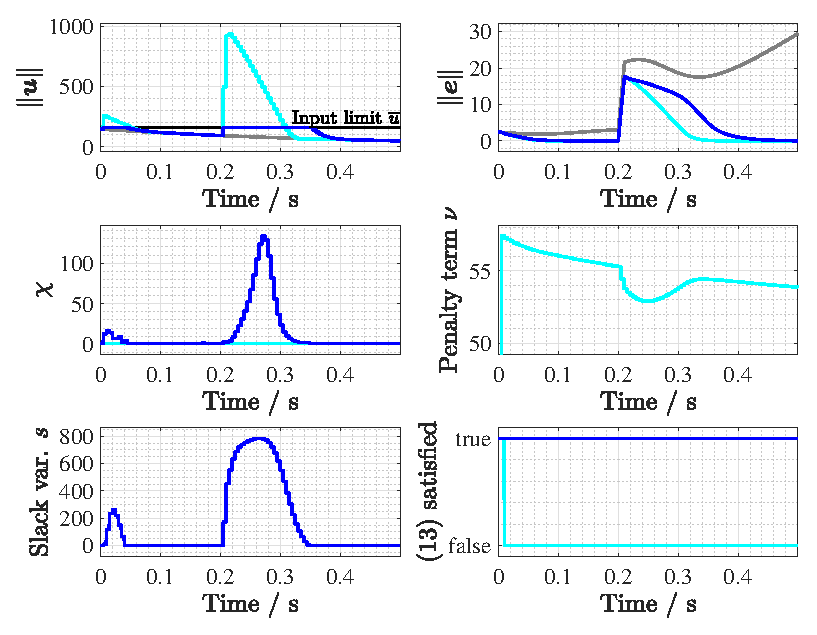
\includegraphics[width=0.99\linewidth]
      {
         src/figures/compare/Fig2.eps
      }
      \label{fig:sim:result:opt}
   }
   \caption{
      Numerical validation results of (C$_1$) \protect\colorLine{blue}{solid}, (C$_2$) \protect\colorLine{my_cyan}{solid}, (C$_3$) \protect\colorLine{gray}{solid}, and desired trajectory $x_d$ \protect\colorLine{red}{dashed}.
      % , and the saturated input of (C$_2$) \protect\colorLine{darkcyan}{solid}.
   }
   \label{fig:sim:result}
\end{figure}

% \begin{figure}[t]
%    \centering
%    \includegraphics[width=0.99\linewidth]
%    {
%       src/figures/compare/Fig1.eps
%    }
%    \caption{
%       Numerical validation results of (C$_1$) \protect\colorLine{blue}{solid}, (C$_2$) \protect\colorLine{my_cyan}{solid}, (C$_3$) \protect\colorLine{gray}{solid}, and desired trajectory $x_d$ \protect\colorLine{red}{dashed}.
%       The saturated input of (C$_2$) is indicated by \protect\colorLine{darkcyan}{solid} in the right-hand side figures
%    }
%    \label{fig:sim:result:control}
% \end{figure}

% \begin{figure}[t]
%    \centering
%    \includegraphics[width=0.99\linewidth]
%    {
%       src/figures/compare/Fig2.eps
%    }
%    \caption{
%       Control input norms, condition numbers, penalty term, and slack variable of (C$_1$) \protect\colorLine{blue}{solid}, (C$_2$) \protect\colorLine{my_cyan}{solid}, and (C$_3$) \protect\colorLine{gray}{solid}.
%    }
%    \label{fig:sim:result:opt}
% \end{figure}

\begin{table}[t]
   \renewcommand{\arraystretch}{1.5}
   \caption{Tracking performances in $L_2$ norm.}
   \centering
   \begin{tabular}{c c c c }
   % \begin{tabular}{c c c c c}
   \hline
   & (C$_1$) \protect\colorLine{blue}{solid} & (C$_2$) \protect\colorLine{my_cyan}{solid} & (C$_3$) \protect\colorLine{gray}{solid} \\
   \hline
   \hline 
   % \multirow{2}{*}{
   $\int_0^T\norm{\mv{e}}\,\der t$
   % } 
   & \oneErr & \twoErr & \threeErr \\
   % & (-\impOne \%)  & (-\impTwo \%) & (–) \\
   \hline
   \end{tabular}
   \label{table:performance}
\end{table}

The numerical validation results are illustrated in Fig.~\ref{fig:sim:result}.
When only the desired controller for nominal model, $\mv{u}=\mv{u}_d$, was applied, \ie (C$_3$), the trajectories of (C$_3$) and $\mv{x}_d$ did not coincide due to the effect of initial condition mismatch.
Significantly, after the disturbance occurrence at $t=0.2$ seconds, the trajectory deviated further from the desired trajectory, as shown in Fig.~\ref{fig:sim:result:control}.

By applying the contraction-based controllers, both (C$_1$) and (C$_2$) successfully drove the trajectory to closely follow the desired trajectory $\mv{x}_d$ even in the presence of disturbances, minimizing the $L_2$ norm of the tracking error to {\oneErr} and {\twoErr}, while (C$_3$) resulted in {\threeErr}, as summarized in Table~\ref{table:performance}.
However, regarding input saturation, (C$_2$) reached the saturation limit due to the initial condition mismatch and the disturbance at $t=0.2$, while (C$_1$) effectively avoided input saturation, as shown in Fig.~\ref{fig:sim:result:opt}.
This demonstrates the effectiveness of the proposed method in handling input saturation constraints while achieving satisfactory tracking performance.

In addition, the expected behavior of the condition number $\chi$, discussed in Section \ref{sec:sub:illustrative}, can be observed for (C$_1$) in Fig.~\ref{fig:sim:result:opt}.
As the contraction constraint \eqref{eq:opt:main:ctrc:proj} and the input saturation constraint \eqref{eq:opt:main:sat} became active, the angle between $\mv{y}$ and $\mv{e}$ increased, resulting in an increase in the condition number to find an unsaturated optimal solution.
Specifically, when the input saturation constraint became active, the condition number $\chi$ increased from $1$ and decreased again to $1$ after the saturation effect disappeared.

In contrast, (C$_2$) kept the smallest condition number, $\chi=1$.
This behavior follows from the objective of \eqref{eq:opt:conv:lmi}, which primarily minimizes the condition number of the contraction metric.
Due to the scale invariance of the condition number, (C$_2$) instead adjusted the scaling factor $\nu$, making $\overline W$ close to the identity matrix and yielding $\mm M=\nu\mm I_n$.
Consequently, the time variation of $\nu$ caused the resulting metric to violate the contraction constraint \eqref{eq:cstr:ctrc}, as shown in Fig.~\ref{fig:sim:result:opt}, as discussed in Section \ref{sec:conv:lmi}.

% As shown in Table~\ref{table:performance}, (C$_2$) achieves better $L_2$ tracking performance than (C$_1$).
% Despite this result, (C$_2$) violates both the contraction constraint \eqref{eq:cstr:ctrc} and the input saturation limit, as shown in Fig.~\ref{fig:sim:result:opt}.
% Thus, although (C$_2$) does not exhibit divergent behavior in this simulation, its contraction-based certificate and input admissibility are not preserved.

Interestingly, the reconstructed contraction metric candidate $\mm{M}$ satisfied the full contraction condition \eqref{eq:cstr:ctrc} during the simulation, as shown in Fig.~\ref{fig:sim:result:opt}, even though the optimization problem \eqref{eq:opt:main} was designed to satisfy only the projected contraction condition \eqref{eq:cstr:ctrc:proj}.
This observation suggests that there may exist sufficient conditions for the projected contraction condition to imply the full contraction certification.

\section{Conclusion} \label{sec:conclusion}

This study presented a vector-space optimization framework based on a projected contraction condition.
By introducing the metric-weighted error vector as a new optimization variable, the proposed method reduces the number of optimization variables, improving scalability.
In addition, it directly handles input saturation constraints that are difficult to incorporate in the conventional LMI framework.
Numerical simulations on the Lorenz system demonstrated satisfactory tracking performance under input saturation.

Future work will study sufficient conditions under which the projected contraction condition implies the full-contraction certification and extend the framework to state constraints and experiments.

% \begin{ack}
% Place acknowledgments here.
% \end{ack}

\bibliography{refs, localRefs}             % bib file to produce the bibliography
                                    % with bibtex (preferred)
\end{document}
